% questions.tex —— 2007 年·普通高等学校招生考试·湖南卷·文科 · 题目内容片段（无答案）
% 由 tools/generate_projects.py 依来源总账自 2007/2007_数学真题_湖南文_试题.md 生成，勿手改（改源 MD 后重跑）


状态：needs-review；依固定候选 PDF 两页（印刷页 381–382）逐题核验，图形已矢量重绘，正式构建与逐页验收见回执。源未列各题分值，不补分值。

\gkpart{一、选择题}

\begin{question}
\gkti{1}不等式 $x^2>x$ 的解集是（　）

（A）$(-\infty,0)$

（B）$(0,1)$

（C）$(1,+\infty)$

（D）$(-\infty,0)\cup(1,+\infty)$

\end{question}
\begin{question}
\gkti{2}若 $O$、$E$、$F$ 是不共线的任意三点，则以下各式中成立的是（　）

（A）$\overrightarrow{EF}=\overrightarrow{OF}+\overrightarrow{OE}$

（B）$\overrightarrow{EF}=\overrightarrow{OF}-\overrightarrow{OE}$

（C）$\overrightarrow{EF}=-\overrightarrow{OF}+\overrightarrow{OE}$

（D）$\overrightarrow{EF}=-\overrightarrow{OF}-\overrightarrow{OE}$

\end{question}
\begin{question}
\gkti{3}设 $p$：$b^2-4ac>0$（$a\neq0$），$q$：关于 $x$ 的方程 $ax^2+bx+c=0$（$a\neq0$）有实根，则 $p$ 是 $q$ 的（　）

（A）充分不必要条件

（B）必要不充分条件

（C）充分必要条件

（D）既不充分也不必要条件

\end{question}
\begin{question}
\gkti{4}在等比数列 $\{a_n\}$（$n\in\mathbf N^*$）中，若 $a_1=1$，$a_4=\dfrac18$，则该数列的前 $10$ 项和为（　）

（A）$2-\dfrac1{2^8}$

（B）$2-\dfrac1{2^9}$

（C）$2-\dfrac1{2^{10}}$

（D）$2-\dfrac1{2^{11}}$

\end{question}
\begin{question}
\gkti{5}在 $(1+x)^n$（$n\in\mathbf N^*$）的二项展开式中，若只有 $x^5$ 的系数最大，则 $n=$（　）

（A）$8$

（B）$9$

（C）$10$

（D）$11$

\Needspace{0.4\textheight}
\end{question}
\begin{question}
\gkti{6}如图，在正四棱柱 $ABCD-A_1B_1C_1D_1$ 中，$E$、$F$ 分别是 $AB_1$、$BC_1$ 的中点，则以下结论中不成立的是（　）
\nopagebreak[4]
\begin{center}% 2007 年湖南卷文科第 6 题：正四棱柱 ABCD-A_1B_1C_1D_1，E、F 分别为 AB_1、BC_1 的中点。
% 来源 PDF：普通高考/2007/2007湖南文.pdf，SHA256 8e889ae321ffa864b24c505b40e7e96956b301487f5a106264b7fcd9f943e068
% 原页：第 1 页（A3 三栏）第 1 栏下部，印刷页 381，图在题干下方。
% 重绘依据：斜投影正方体，A 左下、B 右下、C 右后、D 左后，上底同名加下标 1；
%   可见棱与上底对角线 A_1C_1 实线，被遮棱 D-D_1、C-D、D-A 与上底对角线 B_1D_1 虚线；
%   E 在 AB_1 上、F 在 BC_1 上，均取中点并画小黑点；标注位置按原图。
\begin{tikzpicture}[scale=1.05, semithick,
  every node/.style={inner sep=1.5pt}]
  \coordinate (A)  at (0,0);
  \coordinate (B)  at (2.4,0);
  \coordinate (D)  at (0.9,0.6);
  \coordinate (C)  at (3.3,0.6);
  \coordinate (A1) at (0,2.4);
  \coordinate (B1) at (2.4,2.4);
  \coordinate (D1) at (0.9,3.0);
  \coordinate (C1) at (3.3,3.0);
  % 被遮棱
  \draw[dashed] (D) -- (D1);
  \draw[dashed] (C) -- (D);
  \draw[dashed] (D) -- (A);
  % 可见棱
  \draw (A) -- (B) -- (C) -- (C1) -- (D1) -- (A1) -- cycle;
  \draw (A) -- (A1);
  \draw (B) -- (B1);
  \draw (C) -- (C1);
  \draw (B1) -- (C1);
  \draw (A1) -- (B1);
  % 上底对角线
  \draw (A1) -- (C1);
  \draw[dashed] (B1) -- (D1);
  % 两条侧面对角线（E、F 所在）
  \draw (A) -- (B1);
  \draw (B) -- (C1);
  % E、F
  \coordinate (E) at ($(A)!0.5!(B1)$);
  \coordinate (F) at ($(B)!0.5!(C1)$);
  \fill (E) circle (1.4pt);
  \fill (F) circle (1.4pt);
  \node[anchor=east]  at ([xshift=-2pt]E) {$E$};
  \node[anchor=west]  at ([xshift=2pt]F) {$F$};
  % 顶点标注
  \node[anchor=north east] at (A)  {$A$};
  \node[anchor=north west] at (B)  {$B$};
  \node[anchor=west]       at (C)  {$C$};
  \node[anchor=east]       at (D)  {$D$};
  \node[anchor=south east] at (A1) {$A_1$};
  \node[anchor=south west] at (B1) {$B_1$};
  \node[anchor=south west] at (C1) {$C_1$};
  \node[anchor=south east] at (D1) {$D_1$};
\end{tikzpicture}
\end{center}
\nopagebreak[4]
（A）$EF$ 与 $BB_1$ 垂直

（B）$EF$ 与 $BD$ 垂直

（C）$EF$ 与 $CD$ 异面

（D）$EF$ 与 $A_1C_1$ 异面

\Needspace{0.4\textheight}
\end{question}
\begin{question}
\gkti{7}根据某水文观测点的历史统计数据，得到某条河流水位的频率分布直方图（如图），从图中可以看出，该水文观测点平均至少一百年才遇到一次的洪水的最低水位是（　）
\nopagebreak[4]
\begin{center}% 2007 年湖南卷文科第 7 题：河流水位的频率分布直方图。
% 来源 PDF：普通高考/2007/2007湖南文.pdf，SHA256 8e889ae321ffa864b24c505b40e7e96956b301487f5a106264b7fcd9f943e068
% 原页：第 1 页（A3 三栏）第 2 栏上部，印刷页 381，图在题干下方。
% 重绘依据：横轴水位 30–51 米、组距 1 米；纵轴为频率/组距，标出 0.5%、1%、2% 三条虚线。
%   逐柱高度按原图柱顶量取（以 1% 线为标尺），再按「各组频率之和为 100%」归一：
%   30–31 为 2.6%、31–32 为 3.1%、32–33 为 3.4%，其后渐升，39–40 达峰 8.0%，
%   43–47 有起伏；尾三组按原图标注取 48–49 为 2.0%、49–50 为 1.0%、50–51 为 0.5%。
%   原图只在两端标出 30–33 与 48–51，此处照录。
\begin{tikzpicture}[scale=0.60, semithick, every node/.style={inner sep=1.5pt}]
  % 坐标轴
  \draw[->] (29.7,0) -- (51.9,0) node[anchor=west] {水位（米）};
  \draw[->] (30,0) -- (30,7.6);
  \node[align=center, anchor=south] at (30,7.65) {频率\\[-1pt]组距};
  % 断裂记号
  \draw (29.85,0) -- (29.95,0.12) -- (30.05,-0.02);
  % 三条水平虚线
  \draw[dashed] (30,0.5) -- (51.4,0.5);
  \node[anchor=east] at (29.92,0.5) {$0.5\%$};
  \draw[dashed] (30,1) -- (51.4,1);
  \node[anchor=east] at (29.92,1) {$1\%$};
  \draw[dashed] (30,2) -- (51.4,2);
  \node[anchor=east] at (29.92,2) {$2\%$};
  % 各柱
  \foreach \x/\h in {
    30/2.6, 31/3.1, 32/3.4, 33/3.9, 34/4.5, 35/5.1, 36/5.8,
    37/6.2, 38/6.6, 39/8.0, 40/7.5, 41/6.9, 42/6.3, 43/5.2,
    44/5.8, 45/5.4, 46/5.8, 47/4.8, 48/2.0, 49/1.0, 50/0.5} {
    \draw (\x,\h) rectangle (\x+1,0);
  }
  % 横轴刻度标签（照原图只标两端）
  \foreach \x in {30,31,32,33,48,49,50,51} {
    \node[anchor=north] at (\x,-0.04) {\x};
  }
\end{tikzpicture}
\end{center}
\nopagebreak[4]
（A）$48$ 米

（B）$49$ 米

（C）$50$ 米

（D）$51$ 米

\end{question}
\begin{question}
\gkti{8}函数 $f(x)=\begin{cases}4x-4,&x\leqslant1,\\ x^2-4x+3,&x>1,\end{cases}$ 的图象和函数 $g(x)=\log_2 x$ 的图象的交点个数是（　）

（A）$1$

（B）$2$

（C）$3$

（D）$4$

\end{question}
\begin{question}
\gkti{9}设 $F_1$、$F_2$ 分别是椭圆 $\dfrac{x^2}{a^2}+\dfrac{y^2}{b^2}=1$（$a>b>1$）的左、右焦点，$P$ 是其右准线上纵坐标为 $\sqrt3c$（$c$ 为半焦距）的点，且 $|F_1F_2|=|F_2P|$，则椭圆的离心率是（　）

（A）$\dfrac{\sqrt3-1}{2}$

（B）$\dfrac12$

（C）$\dfrac{\sqrt5-1}{2}$

（D）$\dfrac{\sqrt2}{2}$

\end{question}
\begin{question}
\gkti{10}设集合 $M=\{1,2,3,4,5,6\}$，$S_1$、$S_2$、…、$S_k$ 都是 $M$ 的含两个元素的子集，且满足：对任意的 $S_i=\{a_i,b_i\}$，$S_j=\{a_j,b_j\}$（$i\neq j$，$i$、$j\in\{1,2,3,\cdots,k\}$），都有 $\min\left\{\dfrac{a_i}{b_i},\dfrac{b_i}{a_i}\right\}\neq\min\left\{\dfrac{a_j}{b_j},\dfrac{b_j}{a_j}\right\}$（$\min\{x,y\}$ 表示两个数 $x$、$y$ 中的较小者）．则 $k$ 的最大值是（　）

（A）$10$

（B）$11$

（C）$12$

（D）$13$

\end{question}
\gkpart{二、填空题}

\begin{question}
\gkti{11}圆心为 $(1,1)$ 且与直线 $x+y=4$ 相切的圆的方程是\gkblank{}．

\end{question}
\begin{question}
\gkti{12}在 $\triangle ABC$ 中，角 $A$、$B$、$C$ 所对的边分别为 $a$、$b$、$c$，若 $a=1$，$c=\sqrt3$，$C=\dfrac{\pi}{3}$，则 $A=$\gkblank{}．

\end{question}
\begin{question}
\gkti{13}若 $a>0$，$a^{\frac23}=\dfrac49$，则 $\log_{\frac23}a=$\gkblank{}．

\end{question}
\begin{question}
\gkti{14}设集合 $A=\left\{(x,y)\mid y\geqslant|x-2|,\ x\geqslant0\right\}$，$B=\left\{(x,y)\mid y\leqslant-x+b\right\}$，$A\cap B\neq\varnothing$．

（1）$b$ 的取值范围是\gkblank{}；

（2）若 $(x,y)\in A\cap B$，且 $x+2y$ 的最大值为 $9$，则 $b$ 的值是\gkblank{}．

\end{question}
\begin{question}
\gkti{15}棱长为 $1$ 的正方体 $ABCD-A_1B_1C_1D_1$ 的 $8$ 个顶点都在球 $O$ 的表面上，则球 $O$ 的表面积是\gkblank{}；设 $E$、$F$ 分别是该正方体的棱 $AA_1$、$DD_1$ 的中点，则直线 $EF$ 被球 $O$ 截得的线段长为\gkblank{}．

\end{question}
\begin{question}
\gkti{16}已知函数 $f(x)=1-2\sin^2\left(x+\dfrac{\pi}{8}\right)+2\sin\left(x+\dfrac{\pi}{8}\right)\cos\left(x+\dfrac{\pi}{8}\right)$．求：

（1）函数 $f(x)$ 的最小正周期；

（2）函数 $f(x)$ 的单调增区间．

\end{question}
\gkpart{三、解答题}

\begin{question}
\gkti{17}某地区为下岗人员免费提供财会和计算机培训，以提高下岗人员的再就业能力．每名下岗人员可以选择参加一项培训、参加两项培训或不参加培训，已知参加过财会培训的有 $60\%$，参加过计算机培训的有 $75\%$．假设每个人对培训项目的选择是相互独立的，且各人的选择相互之间没有影响．

（1）任选 $1$ 名下岗人员，求该人参加过培训的概率；

（2）任选 $3$ 名下岗人员，求这 $3$ 人中至少有 $2$ 人参加过培训的概率．

\Needspace{0.4\textheight}
\end{question}
\begin{question}
\gkti{18}如图，已知直二面角 $\alpha-PQ-\beta$，$A\in PQ$，$B\in\alpha$，$C\in\beta$，$CA=CB$，$\angle BAP=45^\circ$，直线 $CA$ 和平面 $\alpha$ 所成的角为 $30^\circ$．
\nopagebreak[4]
\begin{center}% 2007 年湖南卷文科第 18 题：直二面角 α-PQ-β，A∈PQ，B∈α，C∈β。
% 来源 PDF：普通高考/2007/2007湖南文.pdf，SHA256 8e889ae321ffa864b24c505b40e7e96956b301487f5a106264b7fcd9f943e068
% 原页：第 2 页（A3 三栏）第 1 栏上部，印刷页 382，图在题干下方。
% 重绘依据：β 画成上半平面（竖直矩形），α 画成下半平面（平行四边形），交线 PQ 水平；
%   P 在左端、A 在 P 右侧、Q 在 A 右侧；C 在 β 内、B 在 α 内；
%   线段 CA、CB、AB 实线，平面轮廓与交线细实线，标注按原图。
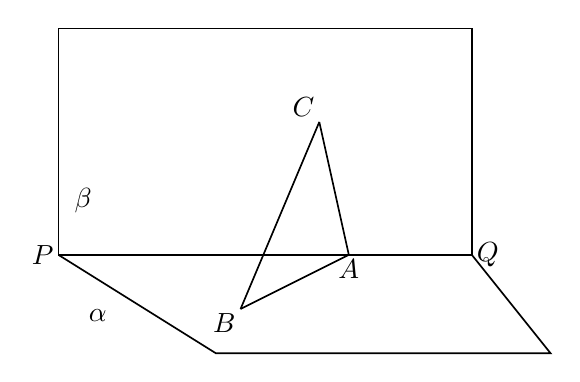
\begin{tikzpicture}[scale=1.25, semithick, every node/.style={inner sep=1.5pt}]
  % 平面 β（上）与 α（下）
  \draw (-2.6,0) -- (1.6,0) -- (1.6,2.3) -- (-2.6,2.3) -- cycle;
  \draw (-2.6,0) -- (-1.0,-1.0) -- (2.4,-1.0) -- (1.6,0);
  % 交线 PQ
  \draw (-2.6,0) -- (1.6,0);
  % 点
  \coordinate (P) at (-2.6,0);
  \coordinate (A) at (0.35,0);
  \coordinate (Q) at (1.6,0);
  \coordinate (C) at (0.05,1.35);
  \coordinate (B) at (-0.75,-0.55);
  % 关键线段
  \draw (C) -- (A);
  \draw (C) -- (B);
  \draw (A) -- (B);
  % 标注
  \node[anchor=east]  at (P) {$P$};
  \node[anchor=north] at (A) {$A$};
  \node[anchor=west]  at (Q) {$Q$};
  \node[anchor=south east] at (C) {$C$};
  \node[anchor=north east] at (B) {$B$};
  \node at (-2.35,0.55) {$\beta$};
  \node at (-2.2,-0.62) {$\alpha$};
\end{tikzpicture}
\end{center}
\nopagebreak[4]
（1）证明：$BC\perp PQ$；

（2）求二面角 $B-AC-P$ 的大小．

\end{question}
\begin{question}
\gkti{19}已知双曲线 $x^2-y^2=2$ 的右焦点为 $F$，过点 $F$ 的动直线与双曲线相交于 $A$、$B$ 两点，点 $C$ 的坐标是 $(1,0)$．

（1）证明：$\overrightarrow{CA}\cdot\overrightarrow{CB}$ 为常数；

（2）若动点 $M$ 满足 $\overrightarrow{CM}=\overrightarrow{CA}+\overrightarrow{CB}+\overrightarrow{CO}$（其中 $O$ 为坐标原点），求点 $M$ 的轨迹方程．

\end{question}
\begin{question}
\gkti{20}设 $S_n$ 是数列 $\{a_n\}$（$n\in\mathbf N^*$）的前 $n$ 项和，$a_1=a$，且 $S_n^2=3n^2a_n+S_{n-1}^2$，$a_n\neq0$，$n=2,3,4,\cdots$．

（1）证明：数列 $\{a_{n+2}-a_n\}$（$n\geqslant2$）是常数数列；

（2）试找出一个奇数 $a$，使以 $18$ 为首项，$7$ 为公比的等比数列 $\{b_n\}$（$n\in\mathbf N^*$）中的所有项都是数列 $\{a_n\}$ 中的项，并指出 $b_n$ 是数列 $\{a_n\}$ 中的第几项．

\end{question}
\begin{question}
\gkti{21}已知函数 $f(x)=\dfrac13x^3+\dfrac12ax^2+bx$ 在区间 $[-1,1)$、$(1,3]$ 内各有一个极值点．

（1）求 $a^2-4b$ 的最大值；

（2）当 $a^2-4b=8$ 时，设函数 $y=f(x)$ 在点 $A(1,f(1))$ 处的切线为 $l$，若 $l$ 在点 $A$ 处穿过 $y=f(x)$ 的图象（即动点在点 $A$ 附近沿曲线 $y=f(x)$ 运动，经过点 $A$ 时，从 $l$ 的一侧进入另一侧），求函数 $f(x)$ 的表达式．

\end{question}